\cleardoublepage
\section{Alignment \label{sec:alignment}}

%%%%%%%%%%%%%%%%%%%%%%%%%%%%%%%%%%%%%%%%%%%%%%%%%%%%%%%%%%%%%%%%%%%%
\subsection{Alignment of the Inner Silicon Tracker}
%%%%%%%%%%%%%%%%%%%%%%%%%%%%%%%%%%%%%%%%%%%%%%%%%%%%%%%%%%%%%%%%%%%%
The determination of the alignment corrections for the Inner Silicon
Tracker to be used for the reprocessing of the 2010 data was done with
the global method~\cite{TkAl_VBlobel,TkAl_Millepede} using a mixture of tracks coming
from atmospheric cosmic rays and minimum bias collisions. 
The global method aligns the highest level structures (half-barrels, endcaps) with all
the six degrees of freedom together with all module units with the most sensitive 
degrees of freedom each: $u$, $w$ and $\gamma$ for the strip modules (also $\alpha$ and $\beta$ in TIB)
and $u$, $v$, $w$ and $\gamma$ for the pixel modules~\footnote{
A local right-handed coordinate system is defined for each module, with $u$ being the
more precisley measured coordinate, $v$ orhogonal to the $u$-axis and in the 
module plane, and the $w$-axis normal to the module plane. Angles $\alpha$, $\beta$ and $\gamma$ are the rotations
around the $u$, $v$ and $w$-axes respectively.}.

During the 2010 LHC run, the geometry of the pixels was monitored on a
daily basis  using the so-called unbiased track-to-primary vertex
residuals. This method consists in selectively
removing a track from the event, determine a primary vertex with the
others, compute the transverse and longitudinal projections of impact
parameter of the probe track with respect the primary vertex and
finally studying the mean value of the distribution of the residuals
as a function of $\phi$, $\eta$ of the track.

Despite starting from a pre-calibrated detector, a discontinuity in
the distribution of the mean longitudinal impact parameter as a
function of azimuthal angle was observed, with the height of the step changing
few times during the year. 
This behavior was interpreted as relative movements, up to 90 $\mu$m in
magnitude, along the $z$-direction of the two BPIX half-barrels,
movements which are allowed since the two halves are mechanically independent.

To cope with this, in a common fit separate sets of alignment corrections for each of
the three BPIX layers in each half-barrel and each of the four FPIX
half-disks in each endcap were provided for seven different periods of
the data-taking. The relative position of the modules with
respect the supporting structure was instead assumed to be the same along all
the 2010 data-taking. 
Figure~\ref{fig:TkAl_PV} shows the distribution of longitudinal separation of the BPIX 
half-barrels as estimated from the unbiased track-to-primary vertex residuals 
as a function of time before and after the alignment procedure. 
 
The statistical precision reached by the alignment was checked looking at the
distribution of the median of the unbiased track-to-hit residuals
computed for each module. 
%In the pixel subsystem, the most relevant component for b-tagging, 
The RMS of these distributions amount to 2 $\mu$m (4 $\mu$m) for the r-$\phi$ ($z$) measurement
coordinate in the BPIX and to 6 $\mu$m (11 $\mu$m) for the r-$\phi$
($r$) measurement in the FPIX, for all the data-taking intervals described above.

A set of alignment parameter errors, calibrated to provide pulls of
the track-to-hit residuals with gaussian standard deviation close to
unity, was provided together with the alignment
constants.

Finally, prior to the restart of the 2011 LHC operations, the alignment
corrections for the two BPIX half-barrels (6 dofs) and for the four FPIX half-disks
(3 translational dofs) were recomputed using a sample of about 15k cosmic ray
tracks.
The analysis of the track-to-primary vertex residuals on events from
2011 collisions indicates that a potentially uncorrected separation of
the two BPIX half-barrels is at most 10 $\mu$m.


%%%%%%%%%%%%%%%%%%%%%%%%%%%%%%%%%%%%%%%%%%%%%%%%%%%%%%%%%%%%%%%%%%%%
\subsection{Simulation-based study of the impact of misalignment on
  b-tagging performances}
%%%%%%%%%%%%%%%%%%%%%%%%%%%%%%%%%%%%%%%%%%%%%%%%%%%%%%%%%%%%%%%%%%%%

The performance of the alignment procedure described above is
essentially not limited by the statistical precision.
To properly describe in the simulation the alignment
accuracy reached at the end of 2010, a misalignment scenario was
prepared following the same approach described in ~\cite{TkAl_CRAFT08}
and using a sample of simulated events with approximately the
same composition of the sample used for the alignment in the data. 
The same alignment parameter errors determined in the data
complemented the misalignment scenario, hereafter referred to as MC2010.

The performances of the different b-tagging algorithms obtained with
the MC2010 misalignment scenario were compared with respect those
obtained with a perfectly aligned detector and with a misalignment
scenario, prepared before the installation of the Inner Silicon Tracker
in CMS, supposed at that epoch to describe the uncertainty on the
alignment parameters expected after 10/pb of collected data~\cite{CMS_NOTE_2008-29}.
The results, obtained from a sample of about 1.5 millions simulated
$t\bar{t}$ events are shown in Figure~\ref{fig:TkAl_effpur_newstartup_vs_ideal}.
For all the taggers the performance with the MC2010 scenario are equal
to those obtained with a perfectly aligned detector.

The same sample of simulated events was used to evaluate the deterioration of the
performances of the b-tagging algorithms in case shifts along the
$z$-direction of the two BPIX half-barrels, similar to those observed
in 2010, were present but not corrected by the alignment procedure.
For this study, the positions and orientations of all the other components of the Tracker 
were supposed to be perfectly known.

Three different scenarios  were investigated
corresponding to 40 $\mu$m, 80 $\mu$m and 160 $\mu$m absolute separation of the
BPIX half-barrels. 
No change in the b-tagging performance is observed for the SSVHE
and SSVHP taggers. For the other taggers
(Figure~\ref{fig:TkAl_effpur_zshifts_vs_ideal}), a significant decrease
of the b-tagging efficiency  is observed only for the 160 $\mu$m separation.
For the track-counting taggers the decrease is more pronounced for 
TCHP, about -5.5\% decrease, already setting-in at the medium
contamination working point, while for the TCHE the decrease is visible
only at the loose contamination working point (about -2.5\% reduction).
In case of the CSVB tagger the decrease is about -2.5\% at 160 $\mu$m separation. 
The largest drop in b-tagging efficiency is observed for the JP and JBP taggers, about -7\%   
at all the tight, medium and loose working points
for the 160 $\mu$m separation scenario.

 

\begin{figure}[!h]
  \centering
    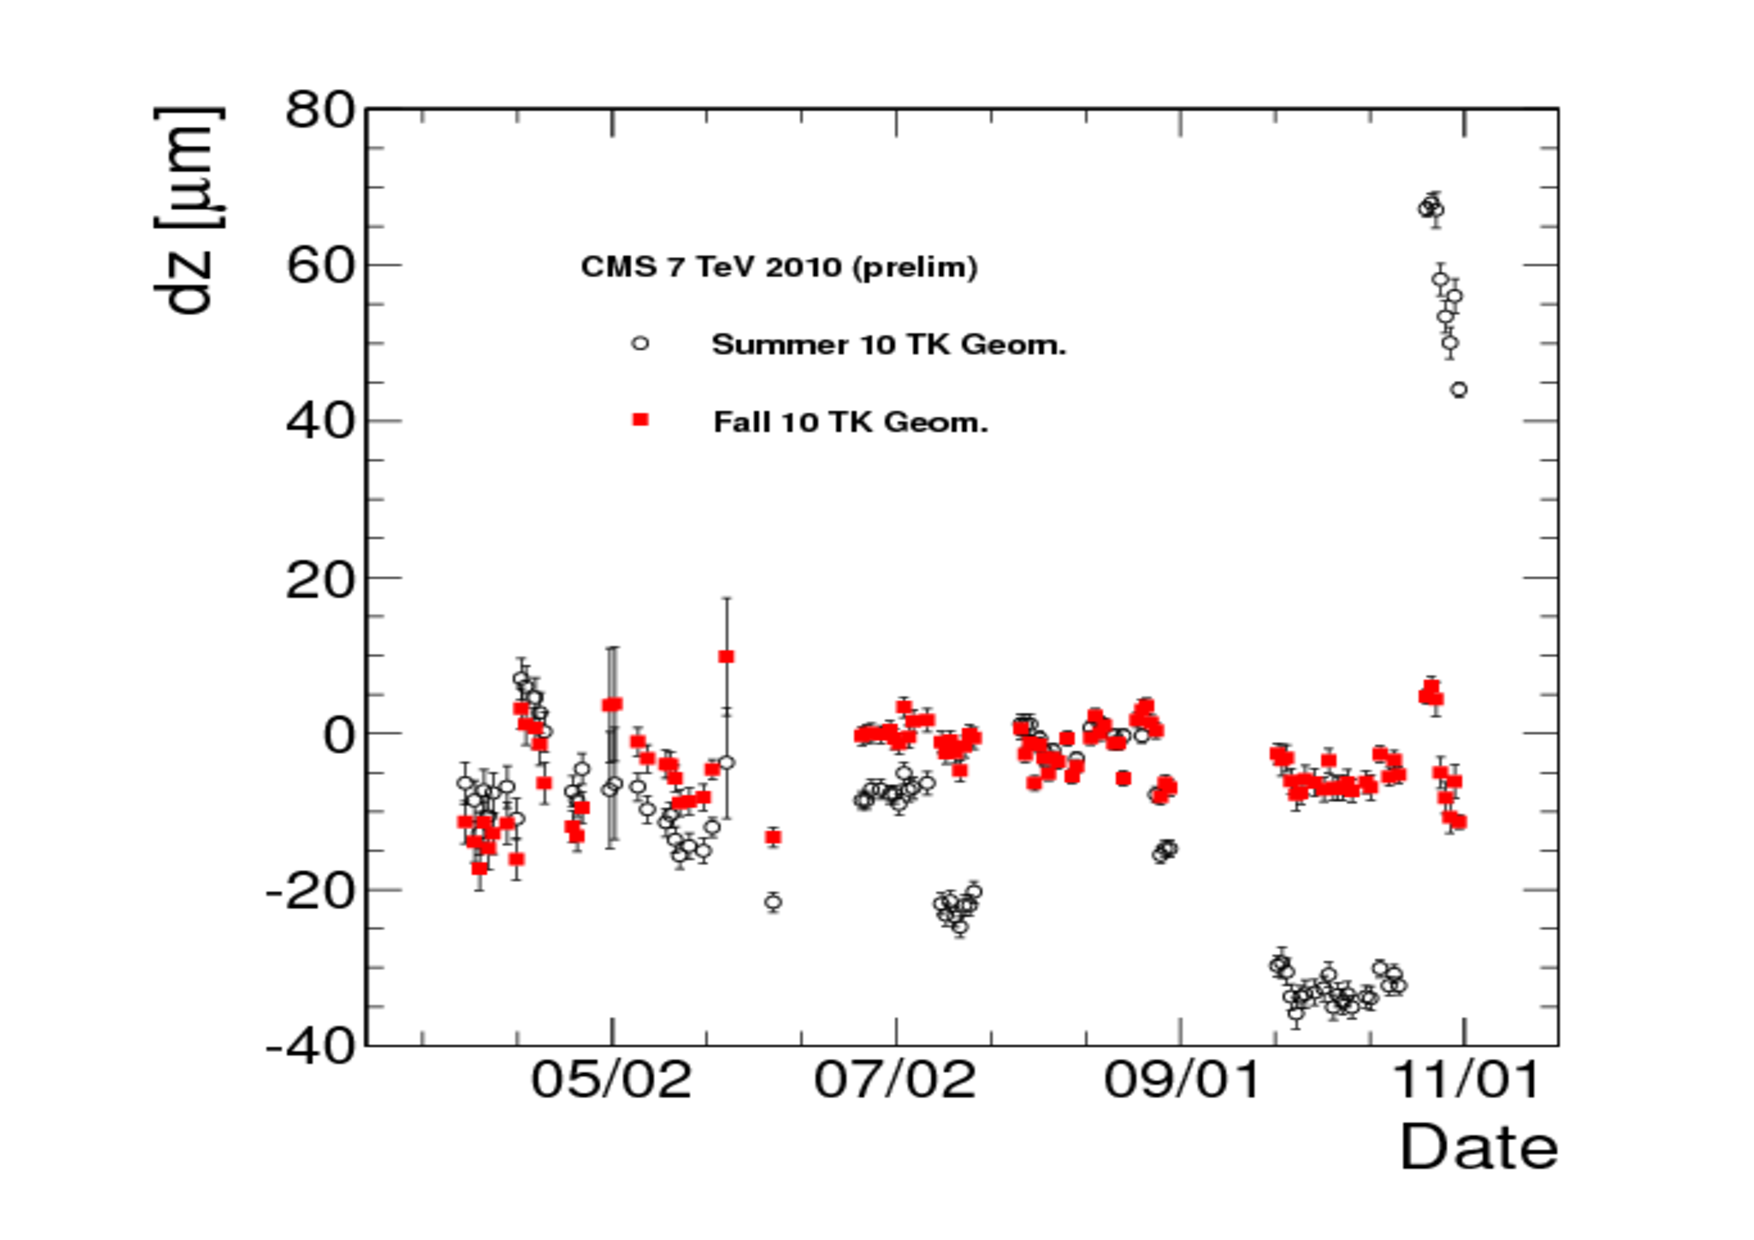
\includegraphics[width=0.7\textwidth]{figures/TkAl_PV}
    \caption{Longitudinal separation of the BPIX half-barrels as
      estimated from the unbiased track-to-primary vertex residual
      method as a function of time for the 2010 LHC proton-proton
      run. Empty (filled) dots are the pre-(post-)alignment values.}
    \label{fig:TkAl_PV}
\end{figure}

\begin{figure}[!h]
  \centering
    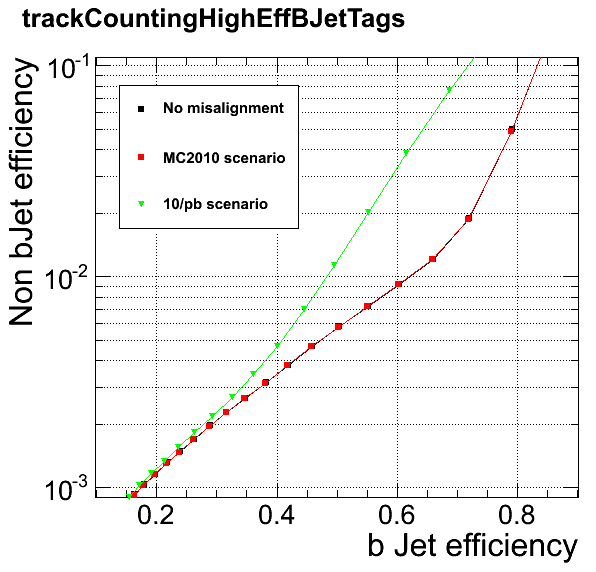
\includegraphics[width=0.45\linewidth]{figures/TkAl_MC2010_TCHE}
    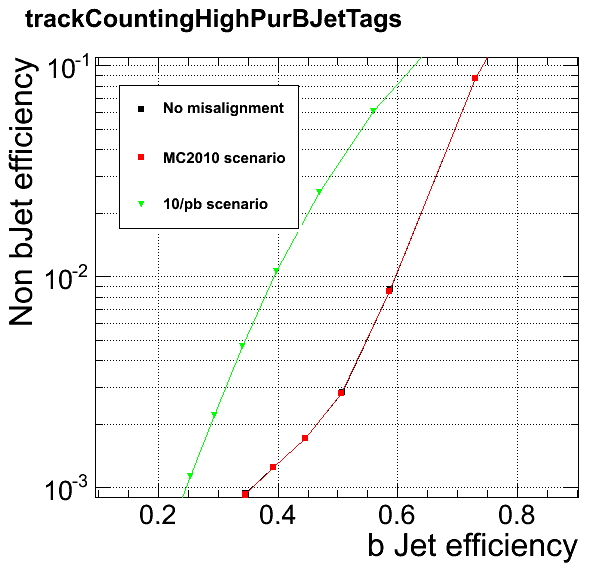
\includegraphics[width=0.45\linewidth]{figures/TkAl_MC2010_TCHP}
    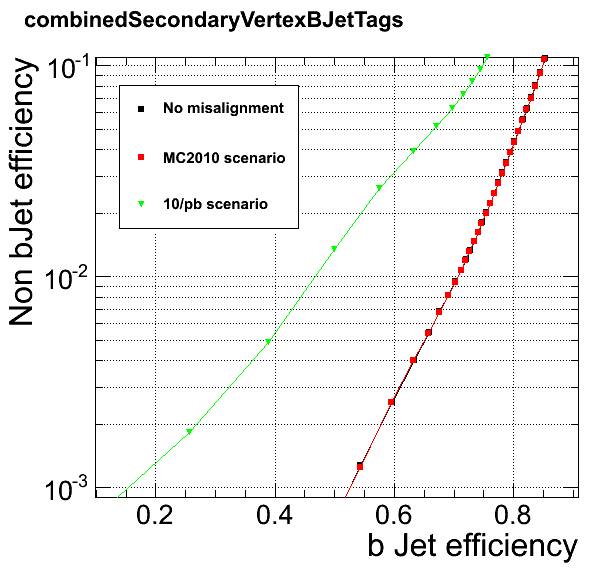
\includegraphics[width=0.45\linewidth]{figures/TkAl_MC2010_CSV}
    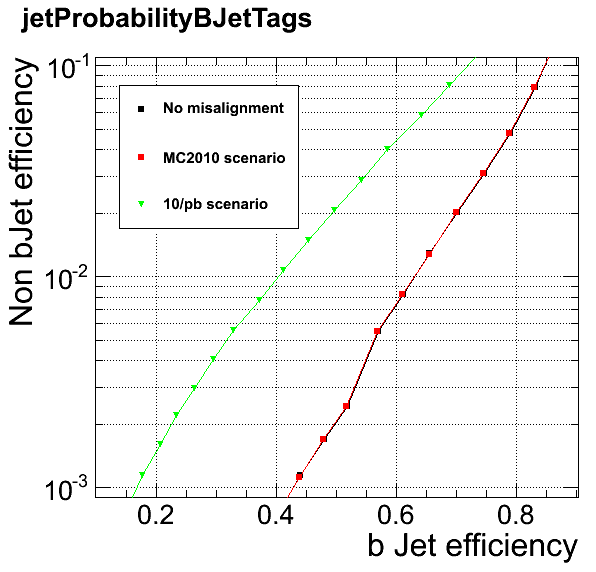
\includegraphics[width=0.45\linewidth]{figures/TkAl_MC2010_JP}
    \caption{Contamination vs. efficiency for the TCHE, TCHP, CSV and JP b-tagging
      algorithms for a scenario describing the estimated current
      accuracy in alignment compared to a perfectly aligned detector.
      For reference the performance expected 
    after 10/pb of collected lumi, based on a previuos study, are also shown.}
    \label{fig:TkAl_effpur_newstartup_vs_ideal}
\end{figure}

\begin{figure}[!h]
  \centering
    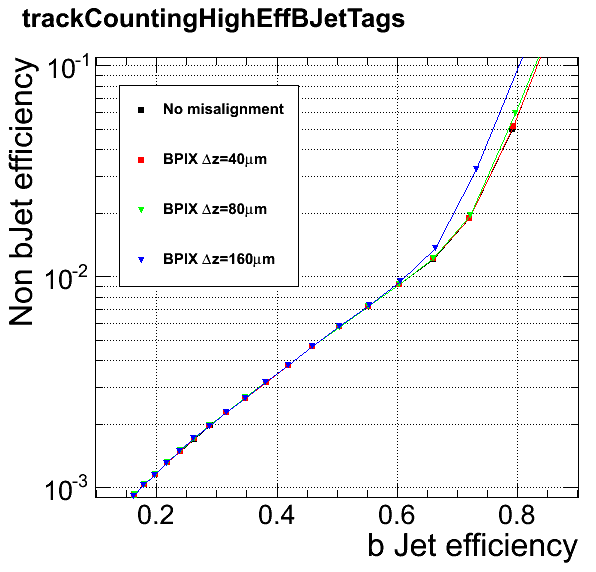
\includegraphics[width=0.45\linewidth]{figures/TkAl_BPIXHBDZ_TCHE}
    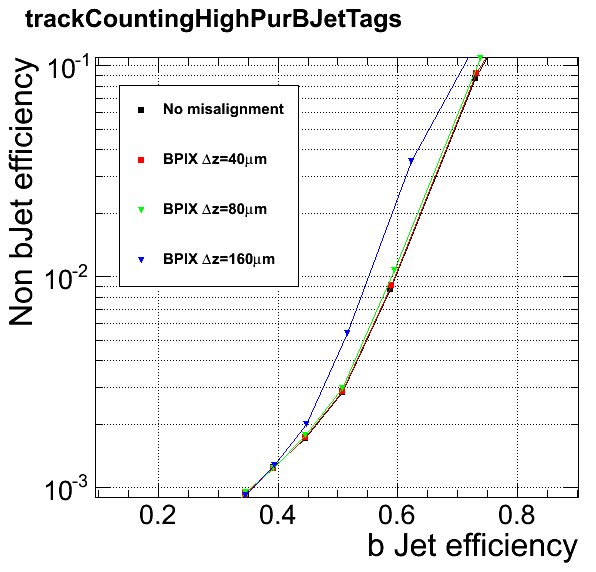
\includegraphics[width=0.45\linewidth]{figures/TkAl_BPIXHBDZ_TCHP}
    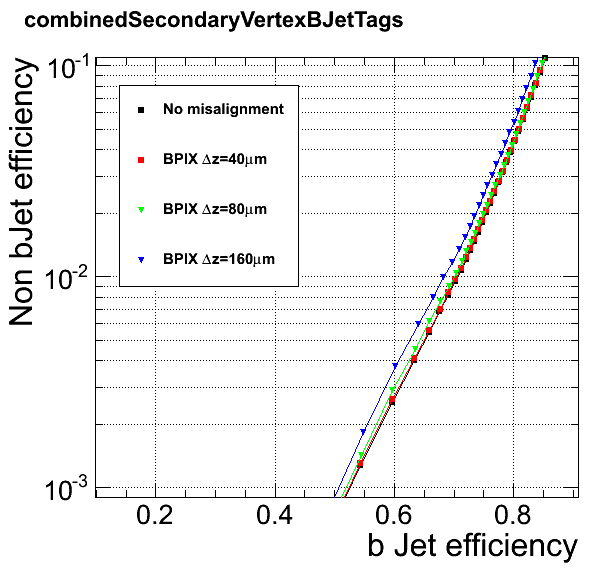
\includegraphics[width=0.45\linewidth]{figures/TkAl_BPIXHBDZ_CSV}
    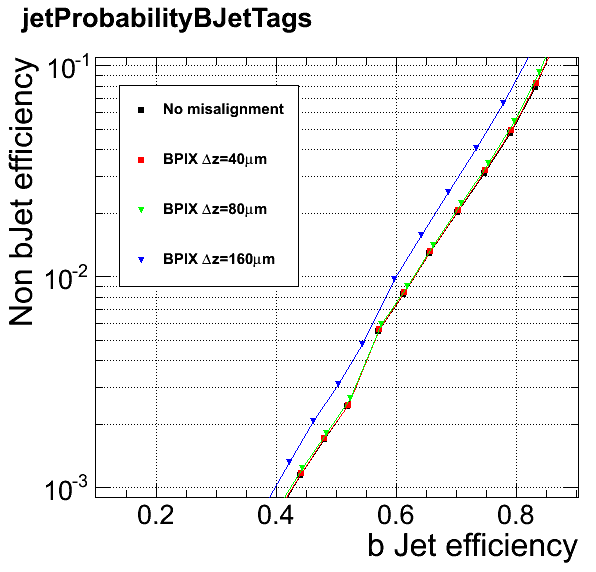
\includegraphics[width=0.45\linewidth]{figures/TkAl_BPIXHBDZ_JP}
    \caption{Contamination vs. efficiency for the TCHE, TCHP, CSV and JP b-tagging
      algorithms for scenarios with an artificial separation of the two BPIX
      half-barrels of 40, 80, 160 $\mu$m.}
    \label{fig:TkAl_effpur_zshifts_vs_ideal}
\end{figure}

